\section{Basic}
    \subsection{prefix sum}
        \lstinputlisting{Basic/prefix_sum.cpp}
    \subsection{difference}
        \lstinputlisting{Basic/difference.cpp}
    \subsection{monotonic queue}
        \lstinputlisting{Basic/monotonic_queue.cpp}
    \subsection{monotonic stack}
        \lstinputlisting{Basic/monotonic_stack.cpp}
    \subsection{kth element}
        \lstinputlisting{Basic/kth_element.cpp}

\section{Graph}
    \subsection{Traversal}
        \lstinputlisting{Graph/traversal.cpp}
    \subsection{Dijkstra}
        \lstinputlisting{Graph/dijkstra.cpp}
    \subsection{Bellman Ford}
        \lstinputlisting{Graph/bellman_ford.cpp}
    \subsection{SPFA}
        \lstinputlisting{Graph/spfa.cpp}
    \subsection{Floyd}
        \lstinputlisting{Graph/floyd.cpp}
    \subsection{Toposort}
        \lstinputlisting{Graph/toposort.cpp}
    \subsection{Kruskal}
        \lstinputlisting{Graph/kruskal.cpp}
    \subsection{差分約束}
        \lstinputlisting{Graph/差分約束.cpp}
    \subsection{LCA}
        \lstinputlisting{Graph/LCA.cpp}
    \subsection{匈牙利算法}
        \lstinputlisting{Graph/匈牙利算法.cpp}
    \subsection{染色法}
        \lstinputlisting{Graph/染色法.cpp}
    \subsection{BCC}
        \lstinputlisting{Graph/BCC.cpp}

\section{Data Structure}
    \subsection{BIT}
        \lstinputlisting{Data structure/BIT.cpp}
    \subsection{DSU}
        \lstinputlisting{Data structure/disjoint_set.cpp}
    \subsection{Segment tree}
        \lstinputlisting{Data structure/segment_tree.cpp}

\section{String}
    \subsection{KMP}
        \lstinputlisting{String/kmp.cpp}
    \subsection{Rabin Karp}
        \lstinputlisting{String/rabin_karp.cpp}
    \subsection{Trie}
        \lstinputlisting{String/trie.cpp}

\section{Math}
	\subsection{extgcd}
		\lstinputlisting{Math/extgcd.cpp}
    \subsection{線性篩}
		\lstinputlisting{Math/線性篩.cpp}
    \subsection{euler}
		\lstinputlisting{Math/euler.cpp}    
    \subsection{guass}
		\lstinputlisting{Math/guass.cpp}
    \subsection{快速冪}
		\lstinputlisting{Math/快速冪.cpp}
    \subsection{模逆元}
		\lstinputlisting{Math/模逆元.cpp}
    \subsection{簡單博弈論}
		\lstinputlisting{Math/簡單博弈論.cpp}
    \subsection{CRT}
        \left\{ 
  \begin{array}{c}
    x \equiv a_1 (mod \; m_1) \\ 
    x \equiv a_2 (mod \; m_2) \\ 
    ... \\
    x \equiv a_k (mod \; m_k)
  \end{array}
\right.

x = a_1M_1M^{-1}_1 + a_2M_2M^{-1}_2 + .. +a_kM_kM^{-1}_k

M = m_1m_2...m_k

M_i = \frac{M}{m_i}
    \subsection{卡特蘭數}
        C^n_{2n} - C^{n-1}_{2n}
= \frac{(2n)!}{n!n!} - \frac{(2n)!}{(n+1)!(n-1)!}
= \frac{(2n)!(n+1) - (2n)!n}{(n+1)!n!}
= \frac{(2n)!}{(n+1)!n!}
= \frac{1}{n+1} \times \frac{(2n)!}{n!n!}
= \frac{C^n_{2n}}{n+1}

\section{Geometry}
    \subsection{Basic}
        \lstinputlisting{Geometry/basic.cpp}

\section{Other}
    \subsection{backpack}
        \lstinputlisting{Other/backpack.cpp}
    \subsection{cmp}
        \lstinputlisting{Other/cmp.cpp}
    \subsection{Python}
        \lstinputlisting{Other/python.py}


\onecolumn
\centering
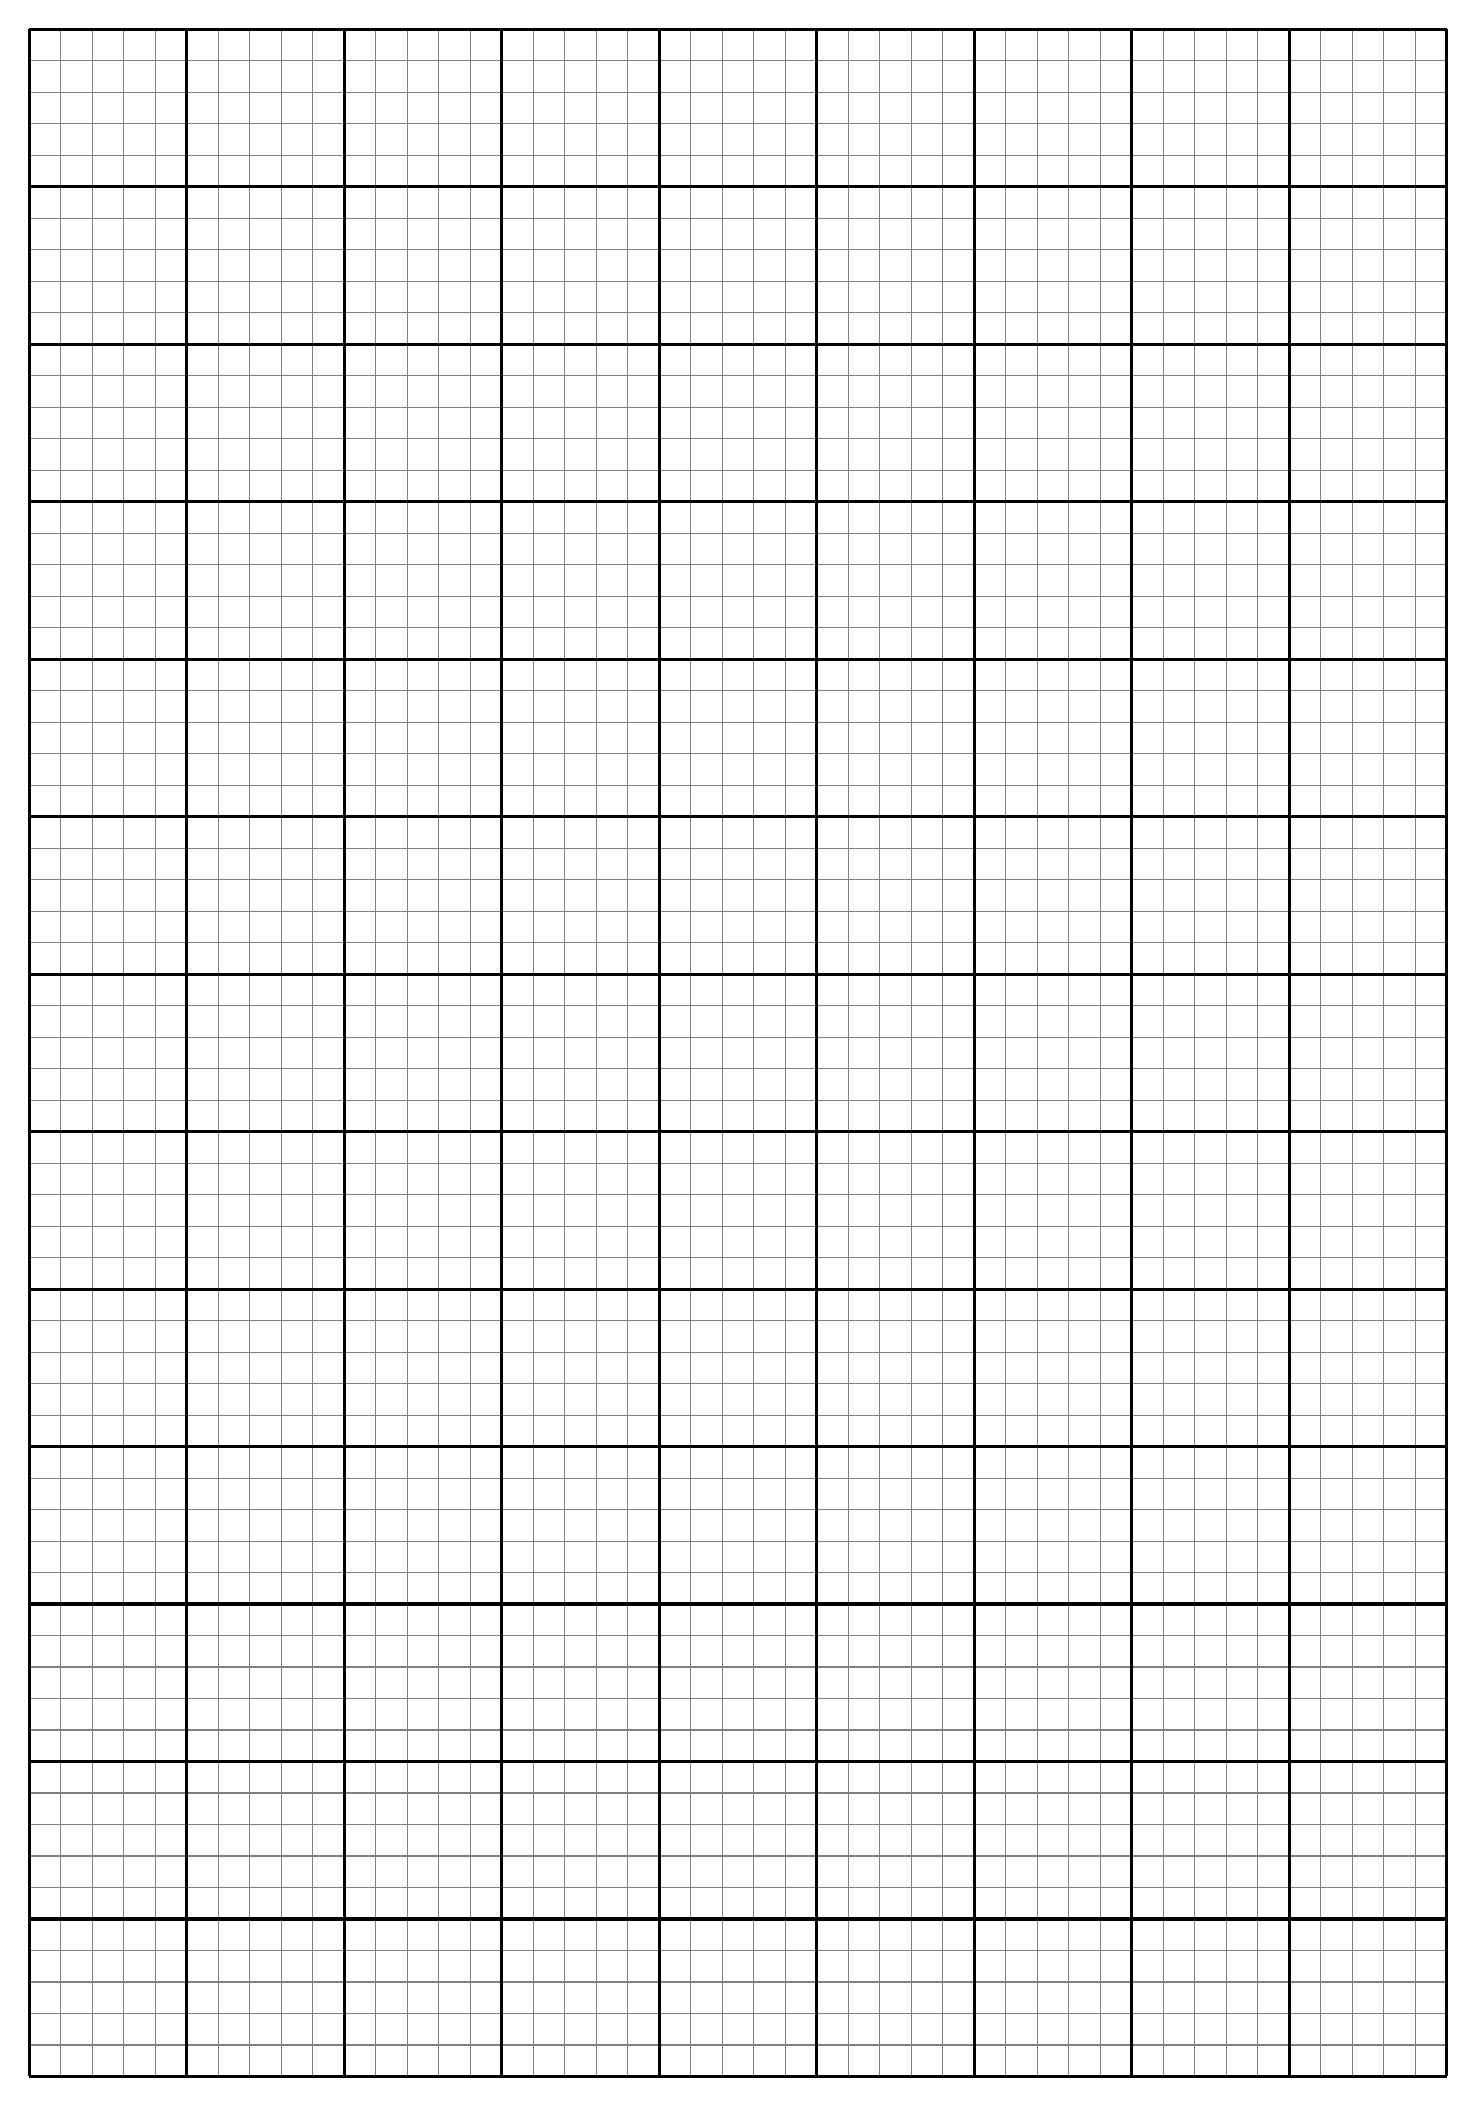
\begin{tikzpicture}[every node/.style={minimum size=1cm-\pgflinewidth, outer sep=10pt}, scale=2]
    \draw[step=0.2cm,color=gray] (0,0) grid (9,13);
    \draw[step=1cm,color=black,line width=0.4mm] (0,0) grid (9,13);
\end{tikzpicture}

\centering
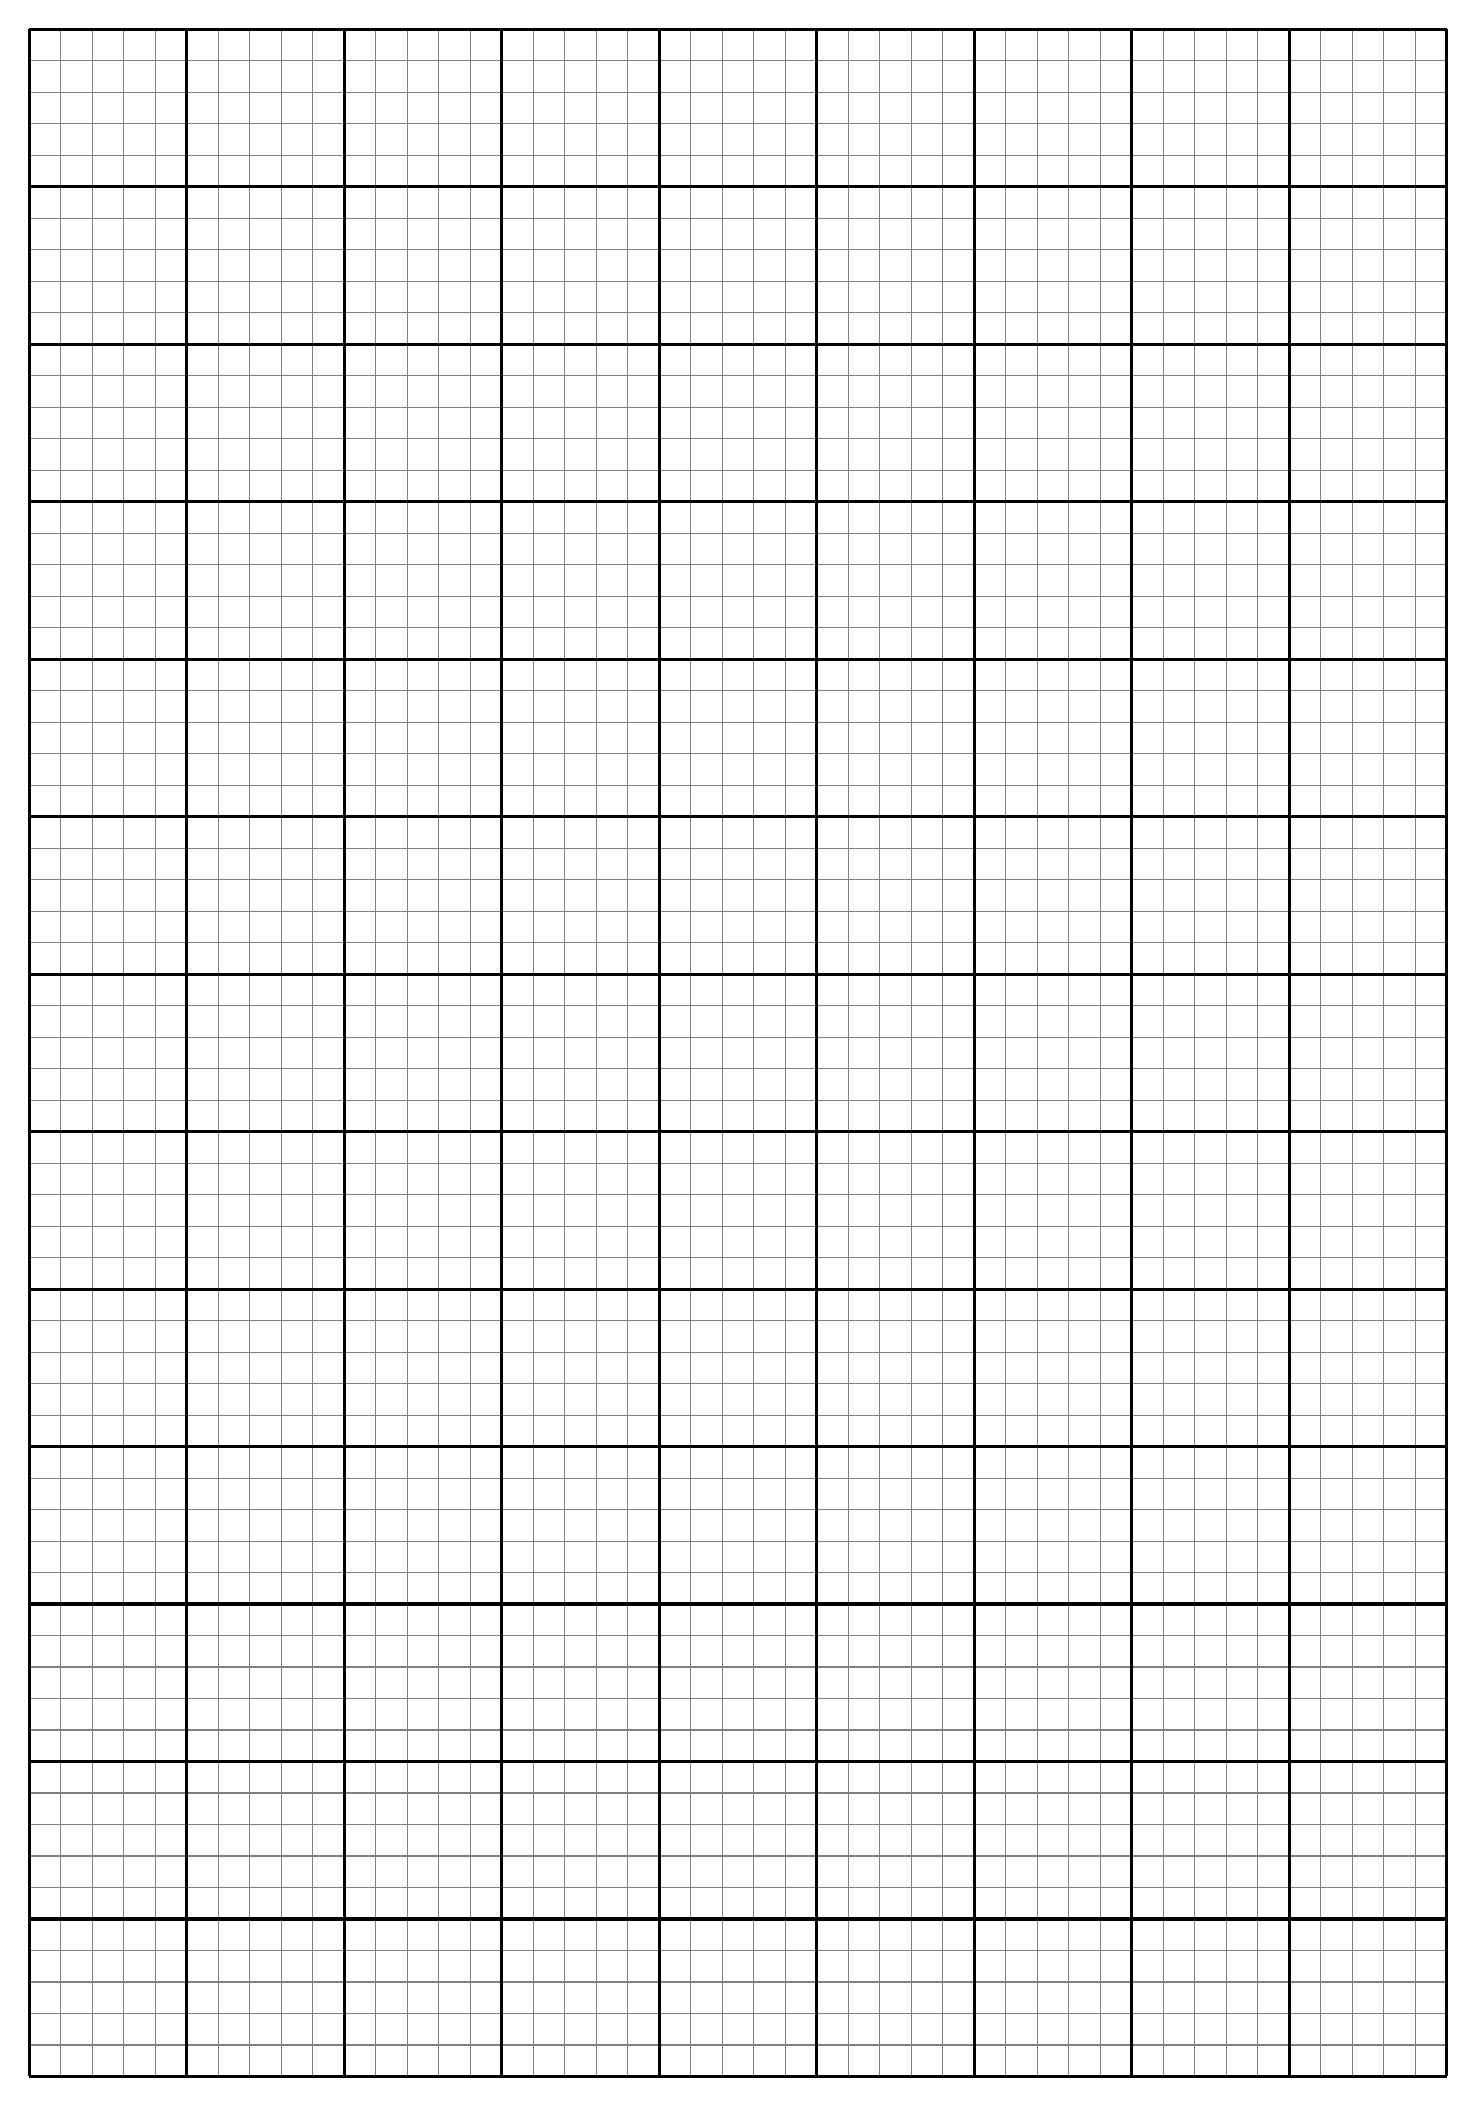
\begin{tikzpicture}[every node/.style={minimum size=1cm-\pgflinewidth, outer sep=10pt}, scale=2]
    \draw[step=0.2cm,color=gray] (0,0) grid (9,13);
    \draw[step=1cm,color=black,line width=0.4mm] (0,0) grid (9,13);
\end{tikzpicture}